\chapter{Daten}\label{ch:daten}

In diesem Kapitel wird zunächst die Wahl der Datenquelle erläutert, anschließend wird die konkrete Erzeugung des Ausgangsdatensatzes beschrieben.
Außerdem wird schrittweise die Verarbeitung des Ausgangsdatensatzes und die daraus resultierende Datenaggregation hin zu einem Evaluations- und Testdatensatzes aufgezeigt.
Der resultierende Datensatz stellt eines der zentralen Ergebnisse dieser Arbeit dar.

% ======================================================================================================================

% Hier wird beschrieben, welche Datenquelle ausgewählt wurde, warum sie ausgewählt wurde und welche Alternativen es gab.
\section{Wahl der Datenquelle}\label{sec:wahl-der-datenquelle}

Um einen Evaluations- und Testdaten zu erzeugen, muss zuerst eine geeignete Datenquelle identifiziert und gegen alternativen abgewogen werden.
Die Datenquelle wird anhand folgender Kriterien ausgewählt:

\begin{itemize}
    \item \textit{Verfügbarkeit} -- die Datenquelle muss für die metaeffekt frei zugänglich sein.
    \item \textit{Realitätsnähe} -- die Datenquelle muss heterogene, reale Daten enthalten, künstliche Daten sollen weitgehend vermieden werden.
    \item \textit{Umfang} -- der Datensatz muss einen für den Anwendungsfall ausreichenden Umfang haben.
    \item \textit{Reproduzierbarkeit} -- der Datensatz soll durch einen reproduzierbaren Prozess erzeugt werden können.
    \item \textit{Erweiterbarkeit} -- der Datensatz soll erweiterbar sein, etwa durch das Hinzufügen weiterer Quellen.
\end{itemize}

% TODO: Quelle einfügen
Eine naheliegende Datenquelle ist das Github Repository des ScanCode-Toolkits, welches einen Testdatensatz zur Erkennung von Copyrights beinhaltet.
Dieser Datensatz besteht aus Quellcode-Dateien und ihren zugehörigen ScanCode-Ergebnissen.
Der Datensatz ist, wie auch das ScanCode-Toolkit, frei verfügbar.
Da es sich in erster Linie um Testdaten für die bestehende Implementierung handelt, bestehen diese zum Teil aus künstlich erzeugten, kuratierten Testfällen, welche nicht klar von realen Daten abgrenzbar sind.
Außerdem ist es schwer einzuschätzen, inwiefern die Testdaten ein reales Spektrum an Copyrights abdecken.
Jedoch ist der Umfang des Testdatensatzes mit mehreren Tausend Dateien ausreichend für die vorgesehene Verwendung (Benchmark und Fine-Tuning).
Der Datensatz wurde manuell kuratiert und entspringt keinem wiederholbaren Prozess, eine Reproduzierbarkeit ist somit nicht gegeben.
Wegen des fehlenden Prozesses ist der Datensatz nur manuell um weitere Quellen erweiterbar.

Die Lizenzdatenbank der metaeffekt \gls{tmd} bietet sich ebenfalls als Datenquelle an.
Sie umfasst über \num{2000} Lizenztexte und ihre metaeffekt-interne Modellierung.
Die Lizenztexte enthalten zwar Copyright-Statements, allerdings dienen diese hauptsächlich als Randfälle, die zur Umsetzung der \nameref{subsec:cep-04} dienen können.
Sowohl die Realitätsnähe als auch die Reproduzierbarkeit und Erweiterbarkeit sind bei dieser Datenquelle kaum gegeben.

Im Laufe der Arbeit wurde eine weitere Datenquelle identifiziert, welche die bisherige Qualität des ScanCode-Toolkit beinhaltet, dabei aber nicht auf künstlichen Daten beruht.
Diese Datenquelle ist ein durch die Prozesse der metaeffekt analysierter und inventarisierter Alpine-Container.
Die Verfügbarkeit der Quelle ist dadurch gegeben, dass der Scan ein Produkt der metaeffekt ist.
Das analysierte Container-Image beinhaltet ausschließlich reale Daten, welche ein breites Spektrum an Paketen und Quellcode beinhalten.
Der Umfang des Scans ist um ein Vielfaches größer als die Testdaten von ScanCode.
Dadurch dass der Scan das Ergebnis eines automatischen Prozesses ist, kann dieser ohne Hindernisse reproduziert und um weitere Scan-Ergebnisse von anderen Quellen erweitert werden.

Anhand der genannten Kriterien wurde der Alpine-Container-Scan als Datenquelle dieser Arbeit gewählt.
Die konkrete Erzeugung dieser Datenquelle wird im nächsten Abschnitt erläutert.

% ======================================================================================================================

\section{Erzeugung des Ausgangsdatensatzes}\label{sec:erzeugung-datensatz}

Beim Scan des Alpine-Containers mithilfe des metaeffekt-Scanners laufen mehrere Schritte ab, die für die Aggregation eines Copyright-Datensatzes relevant sind.
Zunächst werden sämtliche Datenpakete entpackt und die resultierenden Quellcode-Dateien in eines oder mehrere Segmente unterteilt.
Die resultierenden Segmente werden normalisiert und auf diese normalisierten Segmente werden Scan-Prozesse, wie der ScanCode-Service, angewandt.

Das vom ScanCode-Service erzeugte Ergebnis enthält die ermittelten Copyright-Informationen für ein normalisiertes Segment.
Die Normalisierung umfasst unter anderem das Entfernen mehrfacher Leerzeichen sowie von Zeilenumbrüchen.
Die \nameref{subsec:cep-01} besagt, dass Copyright-Statements nicht verändert werden dürfen.
Da die Normalisierung und Segmentierung den originalen Zustand der Datei verändern, können sie nicht für den Datensatz herangezogen werden.
Stattdessen werden die in den Segmenten referenzierten Originaldateien ermittelt und für jede Datei die Scan-Ergebnisse aller ihrer Segmente zusammengeführt.

% TODO: Eventuell hier kurz darauf eingehen, dass der SHA-1 Hash gewählt wurde, um kollisionen zu vermeiden und von originalen Dateinamen zu abstrahieren. Wahrscheinlichkeit für Kollision nennen.
Um Namenskonflikte zu vermeiden, wurde anschließend für jede Originaldatei der SHA-1 Hash berechnet und zusammen mit dem Dateityp zur Benennung der Datei verwendet.
Da die Verzeichnisstruktur der Originaldateien nicht relevant ist, werden alle Dateien in einem flachen Verzeichnis gespeichert, dies vereinfacht die anschließende Verarbeitung zusätzlich.
Der resultierende Ausgangsdatensatz umfasst etwa \num{467000} Originaldateien und ihre Scan-Ergebnisse.

% ======================================================================================================================

\section{Analyse des Datensatzes und Kategorisierung der Daten}\label{sec:analyse-datensatz}

Der erzeugte Datensatz kann in seiner extrahierten Form noch nicht zur Evaluation und Test verwendet werden, da die Scan-Ergebnisse nicht auf den Originaldateien, sondern auf ihren normalisierten Segmenten beruhen.
Um diese Problematik zu adressieren, muss ein Prozess bestimmt werden, der bereits korrekte Daten ermittelt und fehlerhafte Daten, sofern möglich, korrigiert.
Korrekt bedeutet in diesem Kontext, dass die extrahierten Daten der Policy entsprechen.
Dieser Prozess wird nachfolgend schrittweise beschrieben:

\textbf{Schritt 1 -- Unterteilung nach ScanCode-Ergebnissen.}
Der Datensatz wurde in zwei Kategorien unterteilt: Dateien, für die ScanCode \enquote{copyrights}, \enquote{holders} bzw. \enquote{authors} ermitteln konnte, und solche, die keine der genannten Informationen enthalten.
Etwa zwei Drittel des Datensatzes gehören zur letzteren Kategorie.
Die Daten ohne ScanCode-Ergebnis sind allerdings dennoch relevant, da es sich hierbei um False-Negatives des ScanCode-Toolkit handeln kann, die zur Verbesserung der Extraktion unbedingt ermittelt werden müssen.

\textbf{Schritt 2 -- Entfernung von Duplikaten.}
Zunächst wurden Duplikate aus dem Datensatz mit ScanCode-Ergebnissen entfernt.
Hierzu wurden Daten mit demselben SHA-1 Hash ermittelt und alle Duplikate eliminiert.
Diese Filterung reduzierte den Datensatz um etwa 8\,\%.

\textbf{Schritt 3 -- Trennung von Einträgen ohne Copyrights.}
Der von Duplikaten bereinigte Datensatz wurde danach unterteilt, ob das ScanCode-Ergebnis ausschließlich \enquote{authors} enthält.
% TODO: Kategorie von contains no copyrigths zu contains only authors umbenennen.
Diese Kategorie von Daten ohne Copyrights (\enquote{only authors}) umfasst ca.\ 11\,000 Dateien und dient dazu, die Extraktion auf False-Positives beim Erkennen der \enquote{copyrights} zu analysieren.
Außerdem kann dieser Datensatz genutzt werden, das Extrahieren von Autoren gezielt und isoliert zu untersuchen.

\textbf{Schritt 4 -- Abgleich mit Originaldateien (\enquote{exact matches}).}
Die extrahierten Copyright-Statements der ScanCode-Ergebnisse wurden in den entsprechenden Originaldateien gesucht.
Wenn eine Originaldatei jedes der extrahierten Statements exakt enthält, wurde diese Datei und ihr extrahiertes Ergebnis den \enquote{exact matches} zugeordnet.
Das exakte Vorkommen des extrahierten Statements in der Originaldatei erfüllt die Bedingung einer Extraktion \enquote{as-is} gemäß \nameref{subsec:cep-01}.
ScanCode-Ergebnisse, die einen \enquote{exact match} aufweisen und keine Blöcke von Copyrights beinhalten (siehe \nameref{subsec:cep-03}), sind demnach ohne weitere Verarbeitung in Hinsicht auf ihre \enquote{copyrights} Policy-konform.
Blöcke von Copyright-Statements können zwar für jedes extrahierte Statement einen \enquote{exact match} aufweisen, verstoßen aber durch ihre ScanCode bedingte Aufteilung gegen die \nameref{subsec:cep-03}.
Eine korrekte Extraktion der \enquote{holders} und \enquote{authors} erfordert komplexere Mechanismen und wird im Laufe der Arbeit hauptsächlich durch manuelle Überprüfung gewährleistet.
Da die Priorität bei einer korrekten Extraktion der \enquote{copyrights} liegt, werden die möglicherweise fehlerhaft extrahierten Urheber und Autoren als verkraftbares Übel hingenommen.

\textbf{Schritt 5 -- Analyse und Rekonstruktion der \enquote{no exact matches}}
Die ScanCode-Ergebnisse ohne \enquote{exact match} umfassen ca.\ zwei Drittel des Datensatzes.
Die Analyse dieser Ergebnisse zeigte, dass ScanCode unter anderem die Groß- und Kleinschreibung der Statements normalisiert.
Ein Beispiel hierfür ist die konsequente Ersetzung der \enquote{(C)} Markierung durch \enquote{(c)}.
Um diese Fälle zu identifizieren, wurden alle Originaldateien und ihre ScanCode-Ergebnisse in Kleinbuchstaben umgewandelt und anschließend überprüft, ob für jedes extrahierte Statement ein \enquote{exact match} vorliegt.
Wenn ein solcher Match vorlag, konnte geschlussfolgert werden, dass die einzige Differenz zwischen Originaldatei und Extrakt die Groß- bzw.\ Kleinschreibung war.
Dieser Teil des Datensatzes wurde der Kategorie \enquote{exact matches without case} zugeordnet und die enthaltenen Fälle wurden anschließend zu \enquote{exact matches} aufgewertet.
Die Rekonstruktion der Original-Statements erfolgte, indem das extrahierte Statement in der Originaldatei gesucht und anschließend das Original-Statement im Ergebnis ersetzt wurde.
Auf diese Weise konnten ca.\ \num{57000} Dateien den \enquote{exact matches} hinzugefügt werden.

\textbf{Schritt 6 -- Rekonstruktion der Formatierung.}
Da sowohl durch das ScanCode-Toolkit als auch durch die metaeffekt Prozesse Normalisierungen stattfinden, gehen Formatierungen with Zeilenumbrüche und Tabulatoren bzw.\ mehrfache Leerzeichen verloren.
Um die \nameref{subsec:cep-06} zu erfüllen, muss die Formatierung im extrahierten Copyright-Statement erhalten bleiben.
Die durch Normalisierung betroffenen Statements wurden dadurch identifiziert, dass aus den Originaldateien und ScanScode-Ergebnissen jegliche Formatierungen, also Leerzeichen, Zeilenumbrüche und Tabulatoren entfernt wurden.
Anschließend wurde überprüft, ob für jedes Statement einer Datei ein \enquote{exact match} vorliegt.
Die Rekonstruktion dieser \enquote{exact matches without format} erfordert, dass das Statement in der Originaldatei gefunden und anschließend in das ScanCode-Ergebnis kopiert wird.
Da die Statements durch ihre Formatierung nicht eindeutig dem Ergebnis zuweisbar sind, wurde die Levenstein-Distanz zwischen den extrahierten Statements und jedem Substring der Originaldatei berechnet und der Substring gewählt, welcher die geringste Distanz zum Statement ergab.
Anschließend wurden alle Zeichen zwischen dem ersten und letzten Index des Substring aus der Originaldatei in das ScanCode-Ergebnis übertragen.
Durch diese Methode konnten ca.\ \num{6000} \enquote{exact matches without case} rekonstruiert werden.
Die Statements erfordern dennoch Teils manuelle Arbeit, da bei mehrzeiligen Statements die in Kommentarsyntax eingebettet sind, nun auch die entspreche Kommentarsyntax in die Metadaten übertagen wurde.
Die Kategorie \enquote{exact match without format and case} enthält solche Fälle, die sowohl abweichende Formatierung als auch abweichende Groß- und Kleinschreibung im ScanCode-Ergebnis enthalten.
Die Fälle dieser Kategorie wurden dadurch ermittelt, dass zunächst jegliche Formatierung und dann jede Großschreibung in den Originaldateien und den ScanCode-Ergebnissen entfernt wurde, anschließend wurde auch \enquote{exact matches} geprüft.
Von den ursprünglichen rund \num{94000} \enquote{no exact matches} gehören nach den vorherigen Schritten noch ca.\ \num{27000} Dateien der Kategorie \enquote{other reasons} an.
Diese Kategorie erfordert weitere Untersuchungen und eventuell manuelle Aufbereitung.

\textbf{Schritt 7 -- Identifizierung von\enquote{multiple copyrights}.}
Die \enquote{exact matches} wurden danach unterteilt, ob das entsprechende ScanCode-Ergebnis mehrere oder nur ein einzelnes Statement beinhalten.
Die Datei, welche mehrere Statements beinhalten wurde der Kategorie \enquote{multiple copyrights} zugeordnet und anschließend erneut unterteilt, je nachdem ob sie \enquote{authors} enthalten oder nicht.
Die Absicht bei der Unterteilung nach \enquote{multiple copyrights} und die anschließende Unterteilung nach \enquote{authors} soll dazu dienen, dass bei späteren Erstellen von Benchmark bzw.\ Evaluationsdatensätzen möglichst viele Formen von Copyrights in vergleichbarer Anzahl vorhanden sind.
Da die meisten Copyright-Statements im Datensatz einzelne Copyrights ohne Autoren sind, ist es wichtig, keinen Bias aufgrund dieser Datenlage zu erzeugen.

\textbf{Schritt 8 -- Identifizierung von \enquote{single copyrights}.}
Analog zu den \enquote{multiple copyrights} wurden die \enquote{single copyrights} identifiziert und nach dem Vorkommen von \enquote{authors} unterteilt.
Die resultierenden Kategorien \enquote{single copyrights with authors} und \enquote{single copyrights without auhtors} sind die zwei größten Unterkategorien des Datensatzes mit ca.\ \num{20000} Dateien ohne und ca.\ \num{70000} Dateien mit \enquote{authors}.

\textbf{Schritt 9 -- Manuelle Datenpflege.}
Im Laufe dieser Arbeit wurde zu mehreren Zeitpunkten eine Untermenge der Kategorien \enquote{exact matches without format}, \enquote{exact matches without format and case}, \enquote{multiple copyrights}, \enquote{other reasons} und \enquote{only authors} manuell anhand der Policy geprüft und, wenn nötig, korrigiert.
Diese manuell gepflegten Daten wurden regelmäßig dem Stakeholder stichprobenartig zur Validierung vorgelegt und sofern Unregelmäßigkeiten identifiziert wurden, angepasst.
% TODO: hier die finale Zahl der manuellen Datenpflege eintragen und noch auf die Zusammensetzung pro Kategorie eingehen.
Der resultierende Datensatz \enquote{manually checked} umfasst x Dateien und stellt die Kategorie mit der höchsten Qualität in Hinsicht auf die Policy dar.

\begin{figure}[ht]
    \centering
    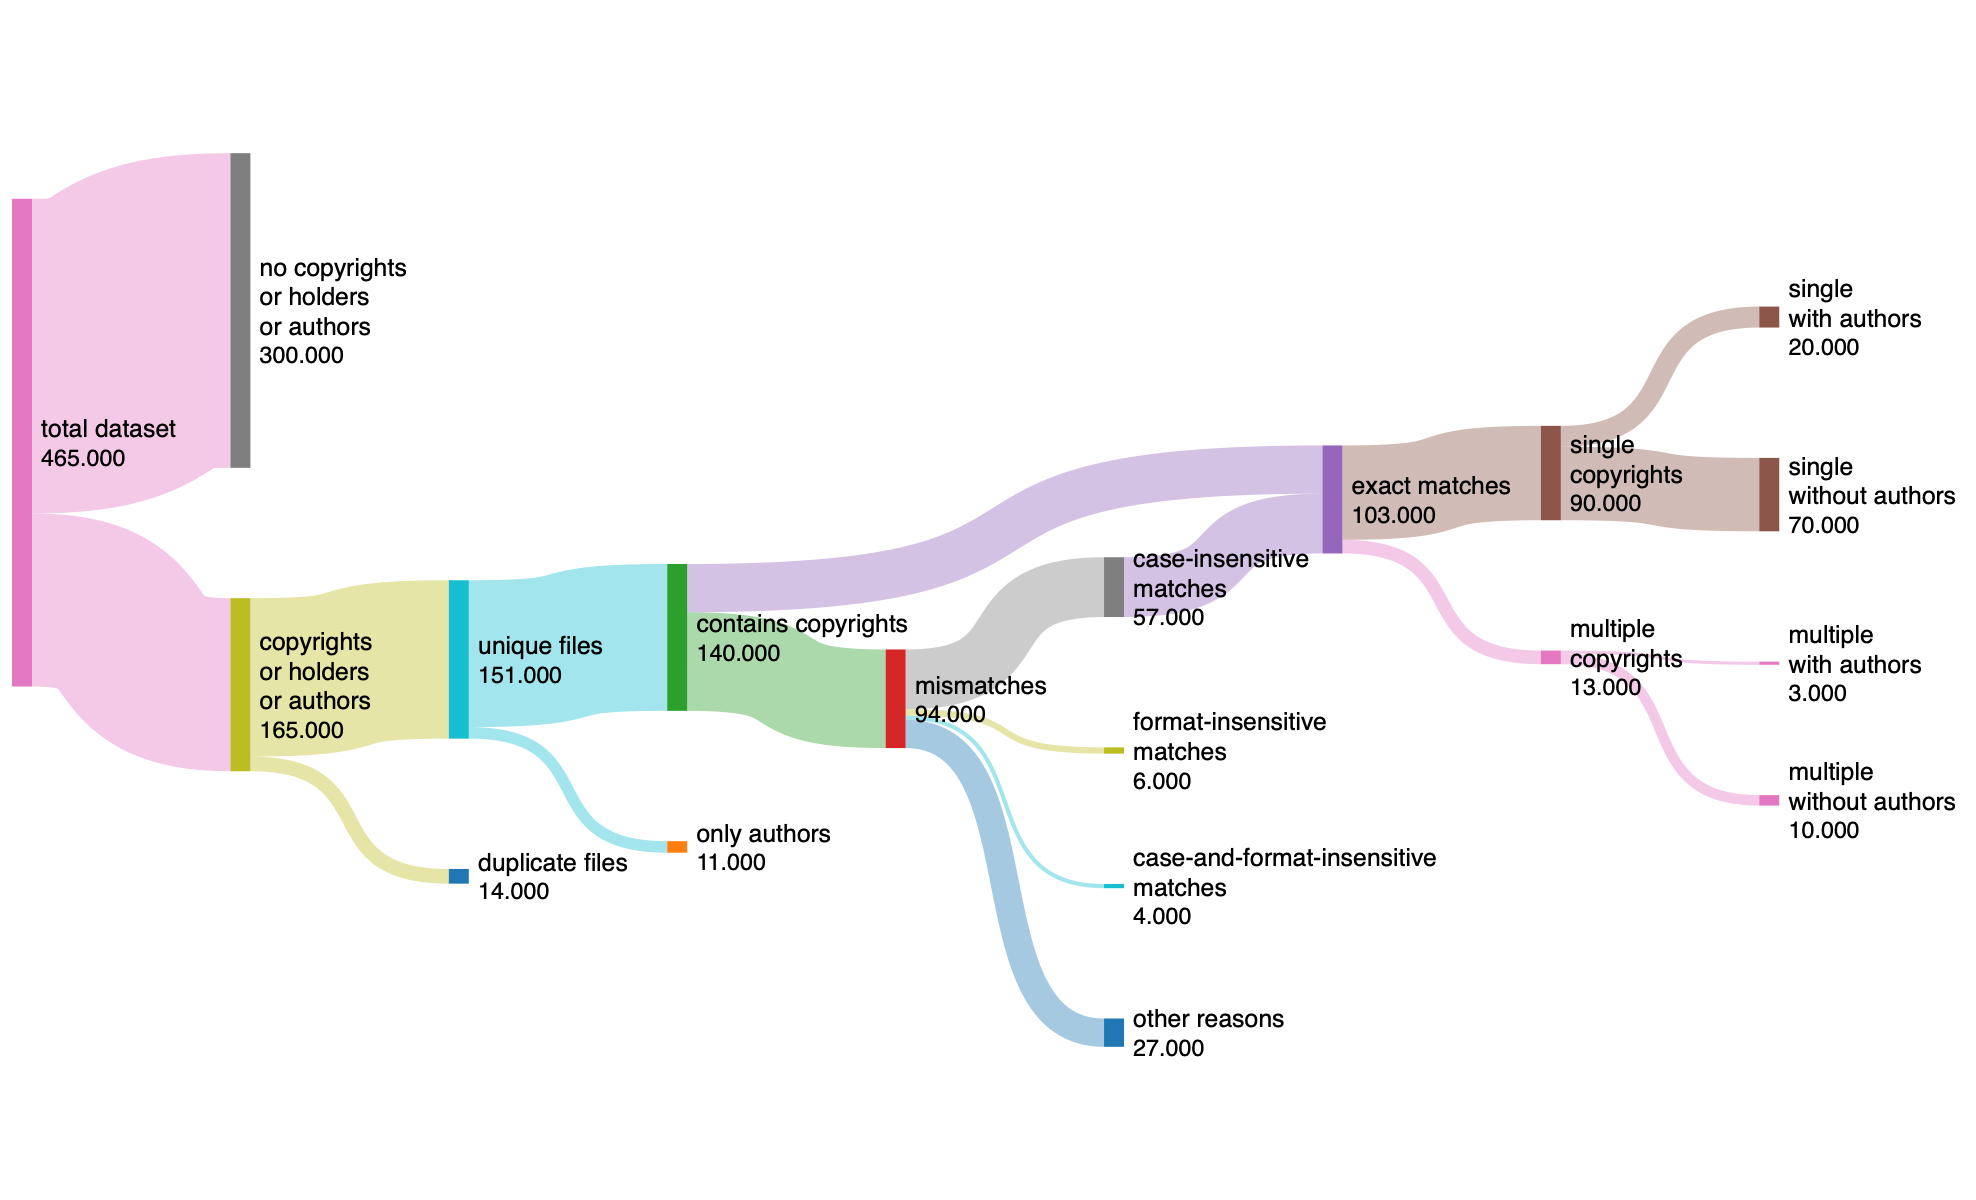
\includegraphics[width=15cm]{daten/data-sankey}
    \caption{Sankey-Diagramm der verschiedenen Kategorien von ScanCode-Ergebnissen bei der Datenaggregation. Das Diagramm veranschaulicht die schrittweise Bildung von Datenkategorien sowie die Anzahl der Quellcode-Dateien pro Zwischenschritt.}
    \label{fig:data-sankey}
\end{figure}
Das Resultat der Datenaggregation sind neun Kategorien von Dateien, welche unterschiedliche Qualitätsstufen in Hinsicht auf die Policy und auf den Aufwand in ihrer Nachbereitung aufweisen.
Die \autoref{fig:data-sankey} veranschaulicht die schrittweise Verarbeitung und Kategorisierung der Daten.
Besonders bei der Abbildung hervorzuheben ist einerseits die Zusammenführung der \enquote{exact matches} und der rekonstruierten \enquote{exact matches without case}, welche den größten Anteil des Datensatzes ausmachen.
Außerdem kann der geneigte Leser anhand der Abbildung erkennen, in welchem Größenverhältnis die verschiedenen Kategorien zueinander stehen bzw.\ welche Kategorien den geringsten Teil des Datensatzes abdecken.
Die aggregierten Kategorien dienen in den folgenden Untersuchungen dazu, möglichst heterogene Testdaten zu wählen und dabei möglichst viele Gestalten von Copyrights zu prüfen.

% ======================================================================================================================

% Hier soll darauf eingegangen werden, welche Probleme und Herausforderungen der Datensatz mit sich gebracht hat, einige
% davon sind die Größe (170GB), die Encodings, Binary-Dateien und die geringe Qualität der Scancode extraktion im "authors" Feld.
\section{Herausforderungen bei der Datenaggregation}\label{sec:herausforderungen-datenaggregation}

Die Verarbeitung der Daten brachte einige Schwierigkeiten mit sich.
Der ursprüngliche Datensatz umfasste ca.\ 170 Gigabyte an Quellcode-Dateien und Metadaten.
Die automatische Analyse einer solchen Datenmenge erfordert robuste Prozesse und zuverlässige, leistungsfähige Hardware.
Eine weitere Herausforderung bei der Verarbeitung der Daten waren die verschiedenen Encodings der Quellcode-Dateien.
Da es sich beim Datensatz um jede Art von Datentyp und Enkodierung handeln kann, muss sichergestellt werden, dass Encodings korrekt erfasst und entsprechend verarbeitet werden.
Im Falle eines nicht klar erkennbaren Encodings wird auf UTF-8 als Default zurückgegriffen.
Neben den Encodings verursachen auch Binär-Dateien zahlreiche Probleme bei der automatischen Auswertung des Datensatzes.
Tritt der Fall auf, dass der Prozess auf eine nicht lesbare Datei stößt, wird diese übersprungen und im weiteren Verlauf nicht berücksichtigt.
Eine verbesserte Version des Datenaggregationsprozesses sollte demnach die korrekte Verarbeitung von Binär-Dateien unterstützen.

% ======================================================================================================================

% Hier soll darauf eingegangen werden, welche Probleme/Qualitätseinbußen der Datensatz aufzuweisen hat, darüber hinaus soll erläutert werden, warum der Datensatz gut ist
% Der Datensatz ist nicht gut weil es keinen besseren gibt -> vielleicht ist ein besserer nur nicht bekannt, stattdessen
% ist der Datensatz mit dem aktuellen Industriestandard (ScanCode) erzeugt worden und wurde nach der von uns erstellten Policy verbessert und validiert
\section{Qualität der Daten}\label{sec:qualitaet-der-daten}

Der aus der Datenaggregation resultierende Datensatz umfasst eine große Anzahl an Dateien die eine Policy-konforme Extraktion von Copyright-Statements aufweisen.
Die \enquote{holders} und \enquote{authors} dieser Extraktionen sind allerdings nicht geprüft und können aus Sicht der Policy fehlerhaft sein.
Einige der Datenkategorien benötigen außerdem noch manuelle Prüfung bzw.\ Pflege.
Um dennoch korrekte Daten dieser Kategorien zur Verfügung zu haben wurde ein manuell überprüfter Datensatz erstellt.
Trotz dieser Qualitätseinbußen ist der generierte und kuratierte Datensatz qualitativ hochwertig.
Die Qualität des Datensatzes ist damit zu begründen, dass der Ausgangsdatensatz mithilfe des Toolkits erzeugt wurde, welches der aktuelle Industriestandard ist, und anschließend in Form der Datenaggregation Schrittweise verbessert wurde.
